\chapter*{GPT-3 : Part 0 - Overview}
\label{chap:gpt3overview}
\thispagestyle{fancy}
\addcontentsline{toc}{chapter}{\nameref{chap:gpt3overview}}

\hspace{0.5cm} Introduced in 2017, The Transformer is a deep learning model primarily used in the field of natural language processing (NLP). Transformers are designed to handle sequential data, such as natural language unlike RNNs, Transformers do not require that the sequential data be processed in order. Thus Transformer allows for much more parallelization than RNNs and therefore reduced training hours. This has led to the development of pre-trained systems such as BERT (Bidirectional Encoder Representations from Transformers) and GPT (Generative Pre-trained Transformer), which have been trained with huge general language datasets, and can be fine-tuned to specific language tasks.

Transformer is an encoder-decoder architecture. The \emph{encoder} consists of a set of encoding layers that processes the input iteratively one layer after another and the \emph{decoder} consists of a set of decoding layers that does the same thing to the output of the encoder. Each encoder and decoder layer makes use of an \emph{attention mechanism}, which for each input, weighs the relevance of every other input and draws information from them accordingly to produce the output. Both the encoder and decoder layers have a feed-forward neural network for additional processing of the outputs, and contain residual connections and layer normalization steps \cite{wiki:transformer} as shown in figure \eqref{fig:trnsfrmarch}.

\begin{figure}[!htbp]
    \centering
    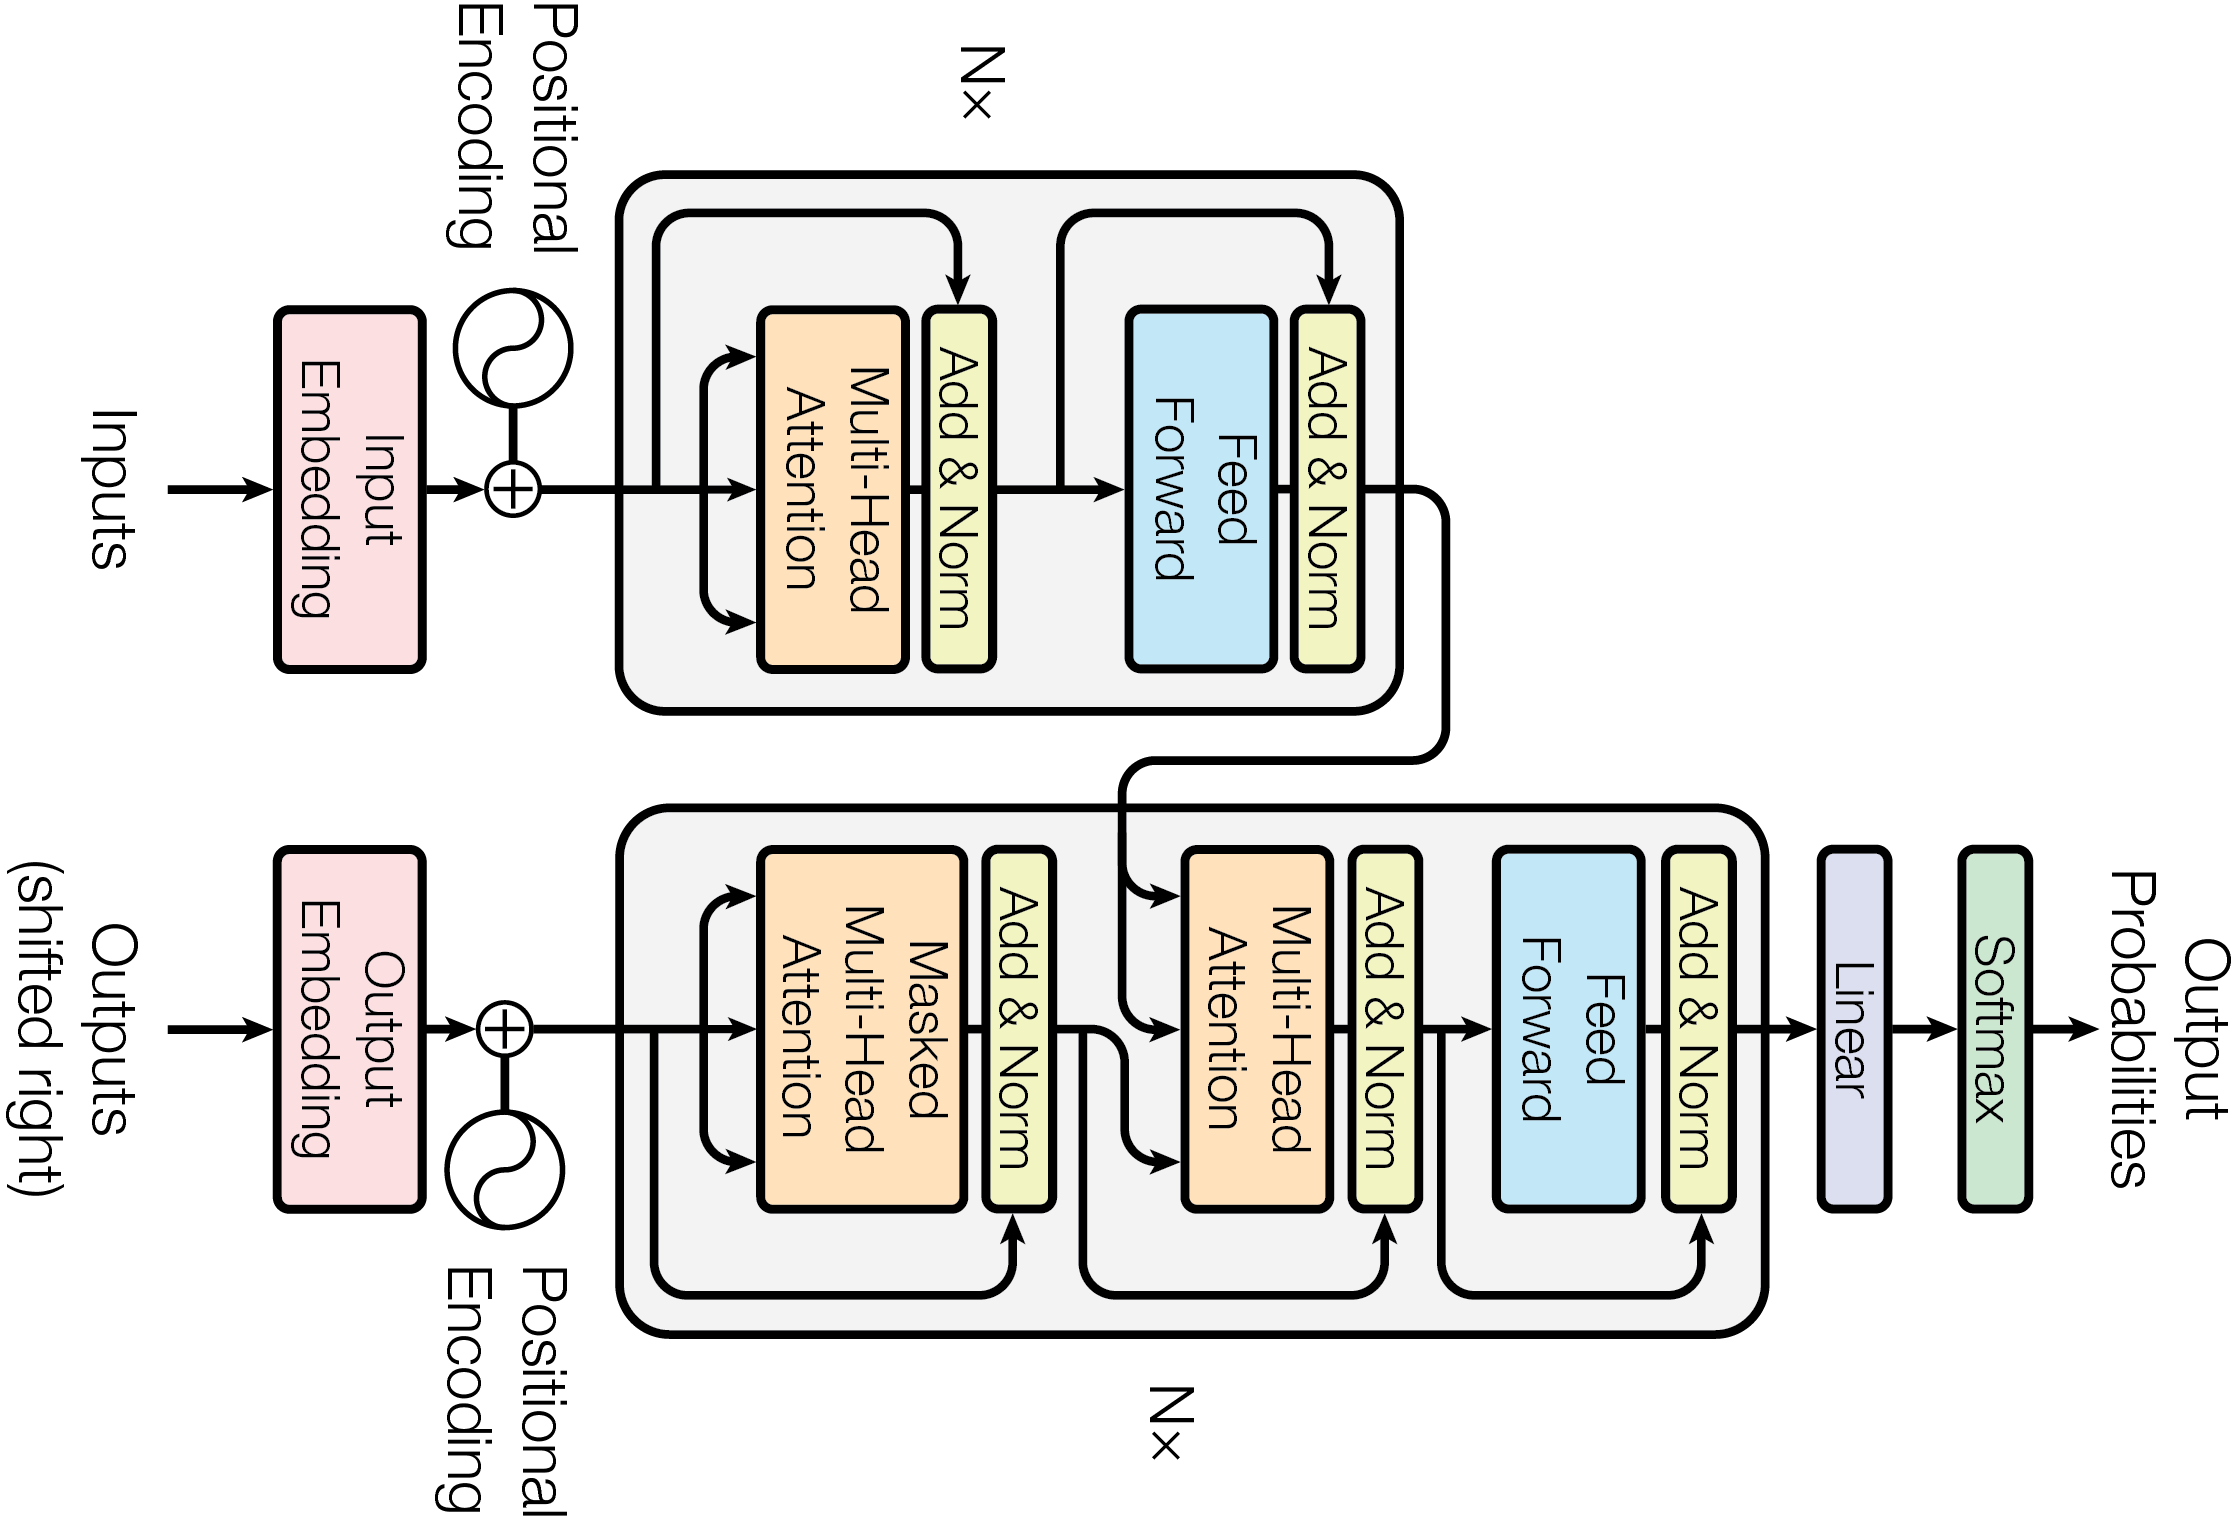
\includegraphics[width=0.7\textwidth]{transformer.png}
    \caption[The Transformer - model architecture]{The Transformer - model architecture \cite{2017arXiv170603762V}}
    \label{fig:trnsfrmarch}
\end{figure}
\vspace*{\fill}
% The basic building blocks of the Transformer are scaled dot-product attention units. When a sentence is passed into a Transformer model, attention weights are calculated between every token simultaneously. The attention unit produces embeddings for every token in context that contain information not only about the token itself, but also a weighted combination of other relevant tokens weighted by the attention weights. Each decoder layer also has an additional attention mechanism which draws information from the outputs of previous decoders, before the decoder layer draws information from the encodings. 